\section{Informes y Estadísticas}

En esta sección se describen los quince informes y estadísticas requeridos para la administración y operación del sistema ECOBICI. Para cada informe se detalla el objetivo de la consulta, seguido del resultado obtenido en la ejecución del script correspondiente.

\subsection{Estadística 1. Daños en bicicletas con mayor frecuencia}

Esta consulta identifica las bicicletas que han estado involucradas en un mayor número de incidentes registrados. La información obtenida permite detectar unidades con problemas recurrentes y apoyar la toma de decisiones relacionadas con mantenimiento preventivo o sustitución de bicicletas.

\begin{figure}[H]
	\centering
	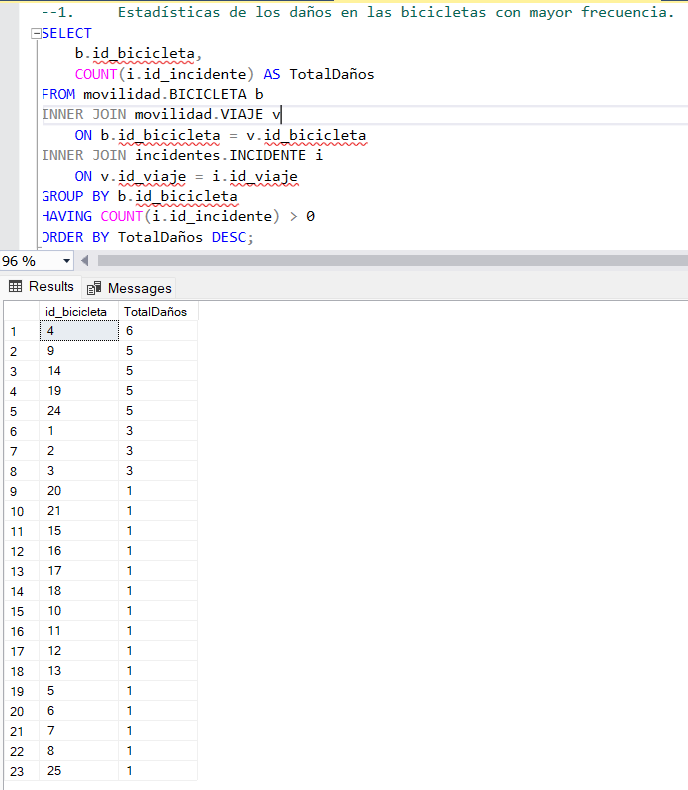
\includegraphics[width=0.85\textwidth]{figures/fig-004.png}
	\caption{Daños en bicicletas con mayor frecuencia}
	\label{fig:est_1}
\end{figure}

\subsection{Estadística 2. Top 5 de accidentes más frecuentes}

Esta consulta muestra los cinco tipos de incidentes que ocurren con mayor frecuencia dentro del sistema ECOBICI. Los resultados permiten identificar los riesgos más comunes y diseñar estrategias de prevención.

\begin{figure}[H]
	\centering
	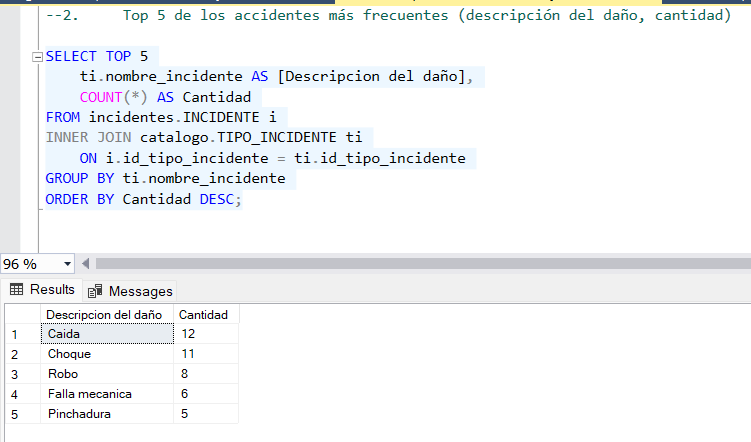
\includegraphics[width=0.85\textwidth]{figures/fig-005.png}
	\caption{Top 5 de accidentes más frecuentes}
	\label{fig:est_2}
\end{figure}

\subsection{Estadística 3. Estaciones con más reportes de accidentes}

Esta consulta presenta las estaciones que registran la mayor cantidad de accidentes durante un periodo determinado, agrupando la información por año y mes. Los resultados ayudan a identificar zonas de mayor riesgo operativo.

\begin{figure}[H]
	\centering
	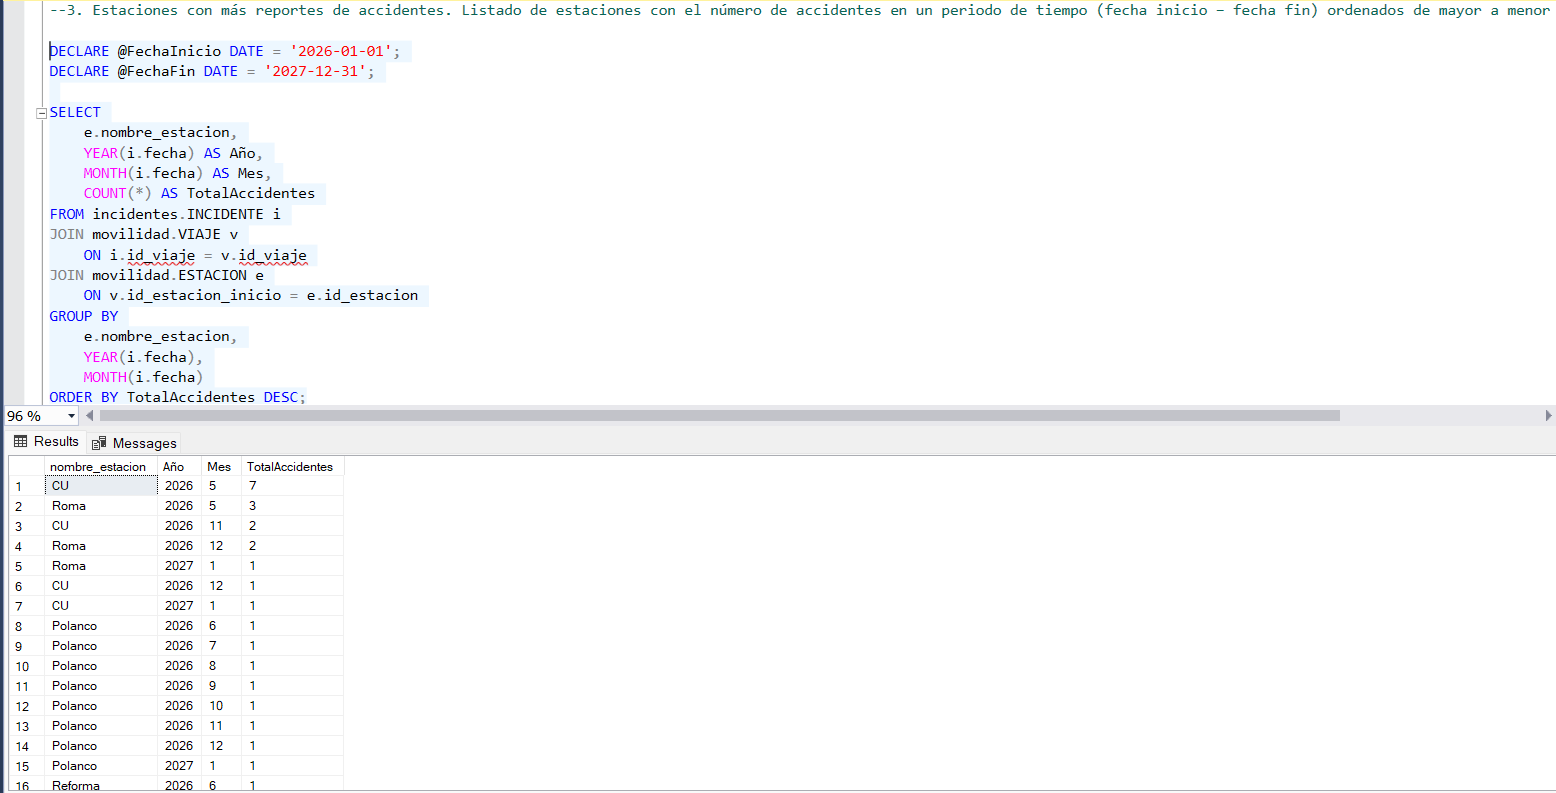
\includegraphics[width=0.85\textwidth]{figures/fig-006.png}
	\caption{Estaciones con más reportes de accidentes}
	\label{fig:est_3}
\end{figure}

\subsection{Estadística 4. Total de accidentes por mes y tipo}

Esta consulta muestra el número de accidentes registrados por mes y tipo de incidente. La información permite analizar tendencias temporales y evaluar el comportamiento de los diferentes tipos de accidentes.

\begin{figure}[H]
	\centering
	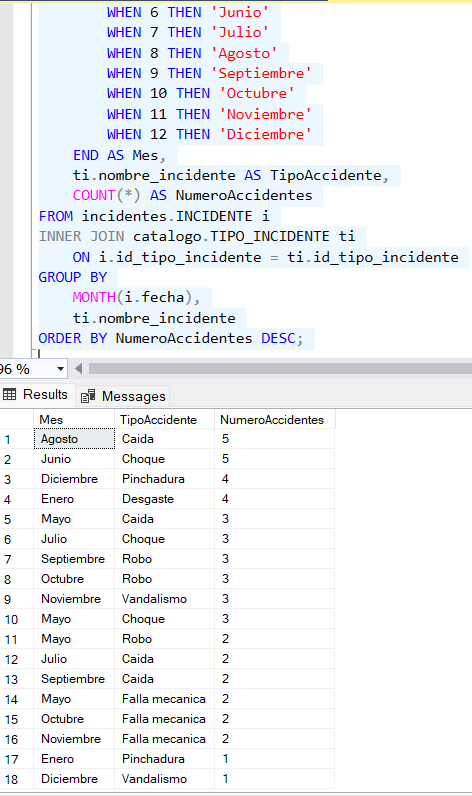
\includegraphics[width=0.85\textwidth]{figures/fig-007.png}
	\caption{Total de accidentes por mes y tipo}
	\label{fig:est_4}
\end{figure}

\subsection{Estadística 5. Usuarios por rango de edad}

Esta consulta clasifica a los usuarios por rangos de edad y tipo de membresía. Su objetivo es conocer la distribución demográfica de los usuarios del sistema.

\begin{figure}[H]
	\centering
	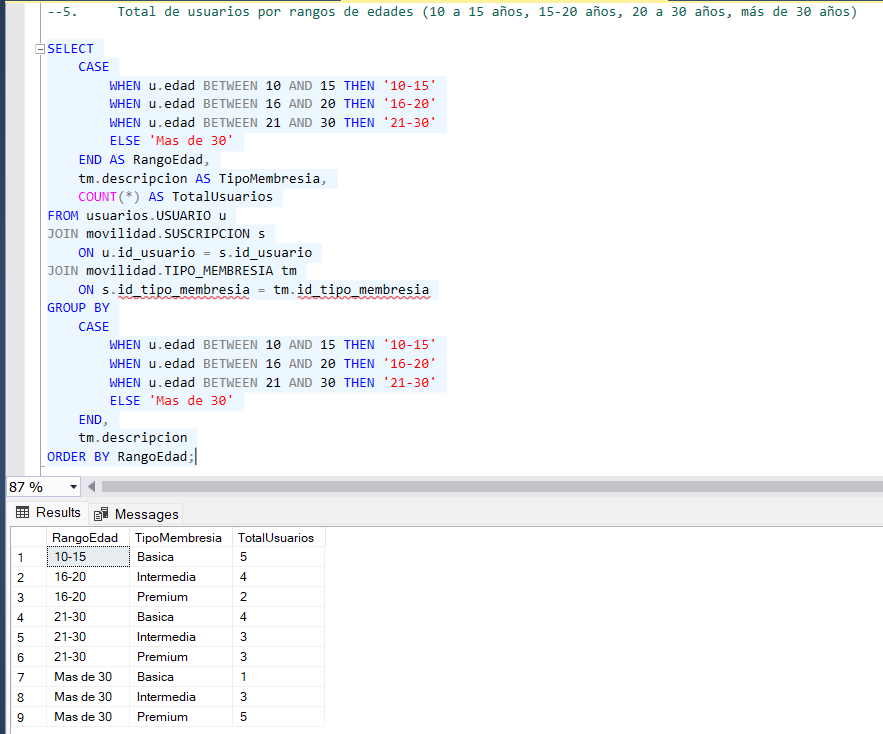
\includegraphics[width=0.85\textwidth]{figures/fig-008.png}
	\caption{Usuarios por rango de edad}
	\label{fig:est_5}
\end{figure}

\subsection{Estadística 6. Inventario de bicicletas por estación}

Esta consulta muestra el inventario de bicicletas por estación, incluyendo estado, color, cantidad de viajes realizados y número de accidentes asociados.

\begin{figure}[H]
	\centering
	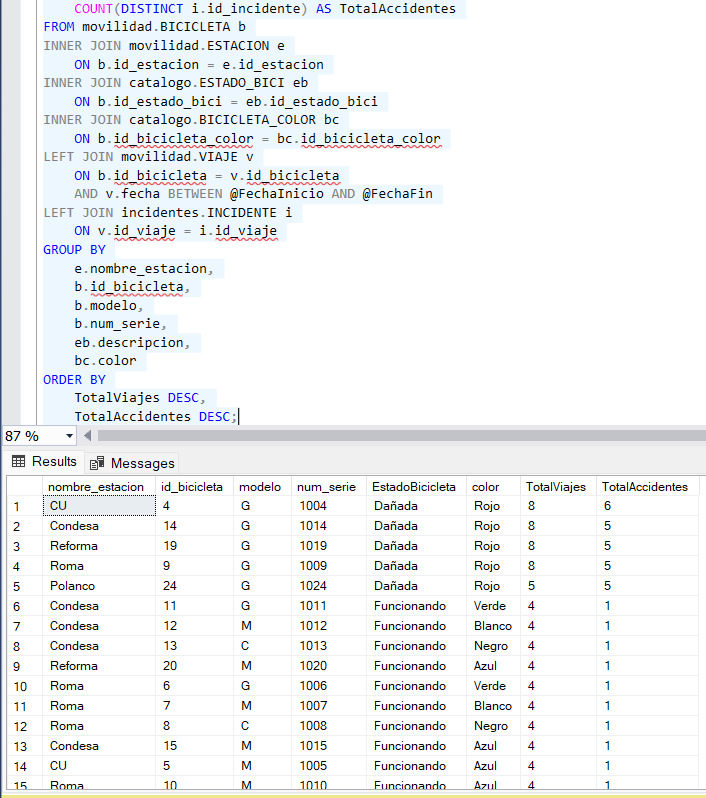
\includegraphics[width=0.85\textwidth]{figures/fig-009.png}
	\caption{Inventario de bicicletas por estación}
	\label{fig:est_6}
\end{figure}

\subsection{Estadística 7. Usuarios y antigüedad de membresía}

Esta consulta presenta la información general de los usuarios, el tipo de membresía que poseen y el tiempo que han permanecido suscritos al servicio en meses.

\begin{figure}[H]
	\centering
	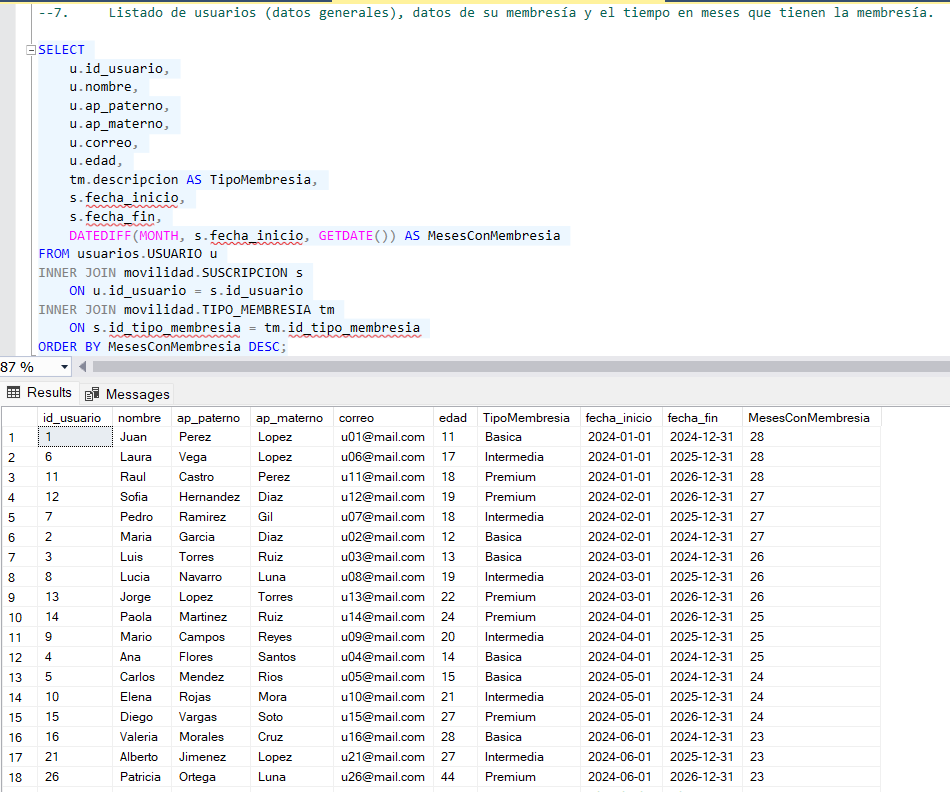
\includegraphics[width=0.85\textwidth]{figures/fig-010.png}
	\caption{Usuarios y antigüedad de membresía}
	\label{fig:est_7}
\end{figure}

\subsection{Estadística 8. Agentes mejor evaluados}

Esta consulta identifica a los agentes con mejor desempeño según las encuestas de satisfacción realizadas por los usuarios después de la atención de incidentes en un mes específico.

\begin{figure}[H]
	\centering
	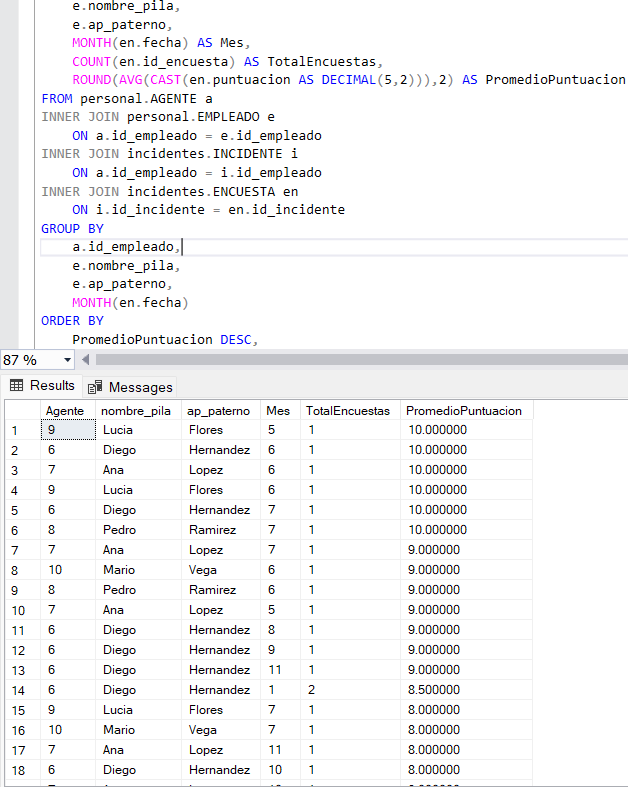
\includegraphics[width=0.85\textwidth]{figures/fig-011.png}
	\caption{Agentes mejor evaluados}
	\label{fig:est_8}
\end{figure}

\subsection{Estadística 9. Reporte diario de rondines}

Esta consulta genera un reporte diario de las actividades realizadas por el personal de rondín, incluyendo incidentes detectados, estación asociada y supervisor responsable (quien también es un empleado de rondines).

\begin{figure}[H]
	\centering
	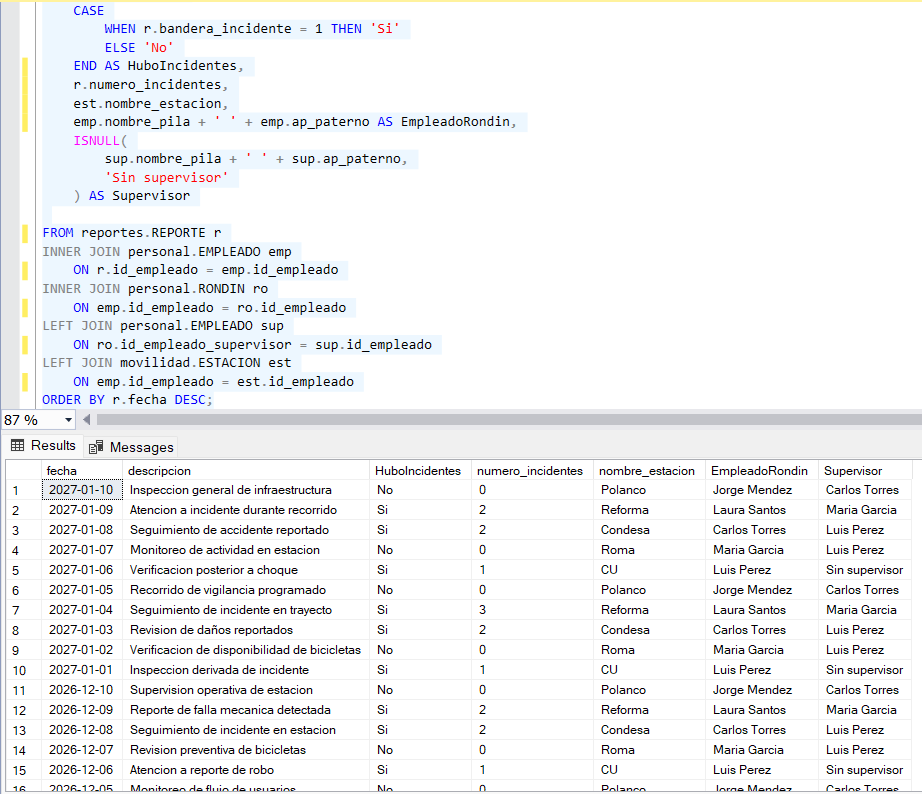
\includegraphics[width=0.85\textwidth]{figures/fig-012.png}
	\caption{Reporte diario de rondines}
	\label{fig:est_9}
\end{figure}

\subsection{Estadística 10. Listado completo de empleados}

Esta consulta muestra la información completa de los empleados registrados en el sistema, indicando además el tipo de puesto que desempeñan.

\begin{figure}[H]
	\centering
	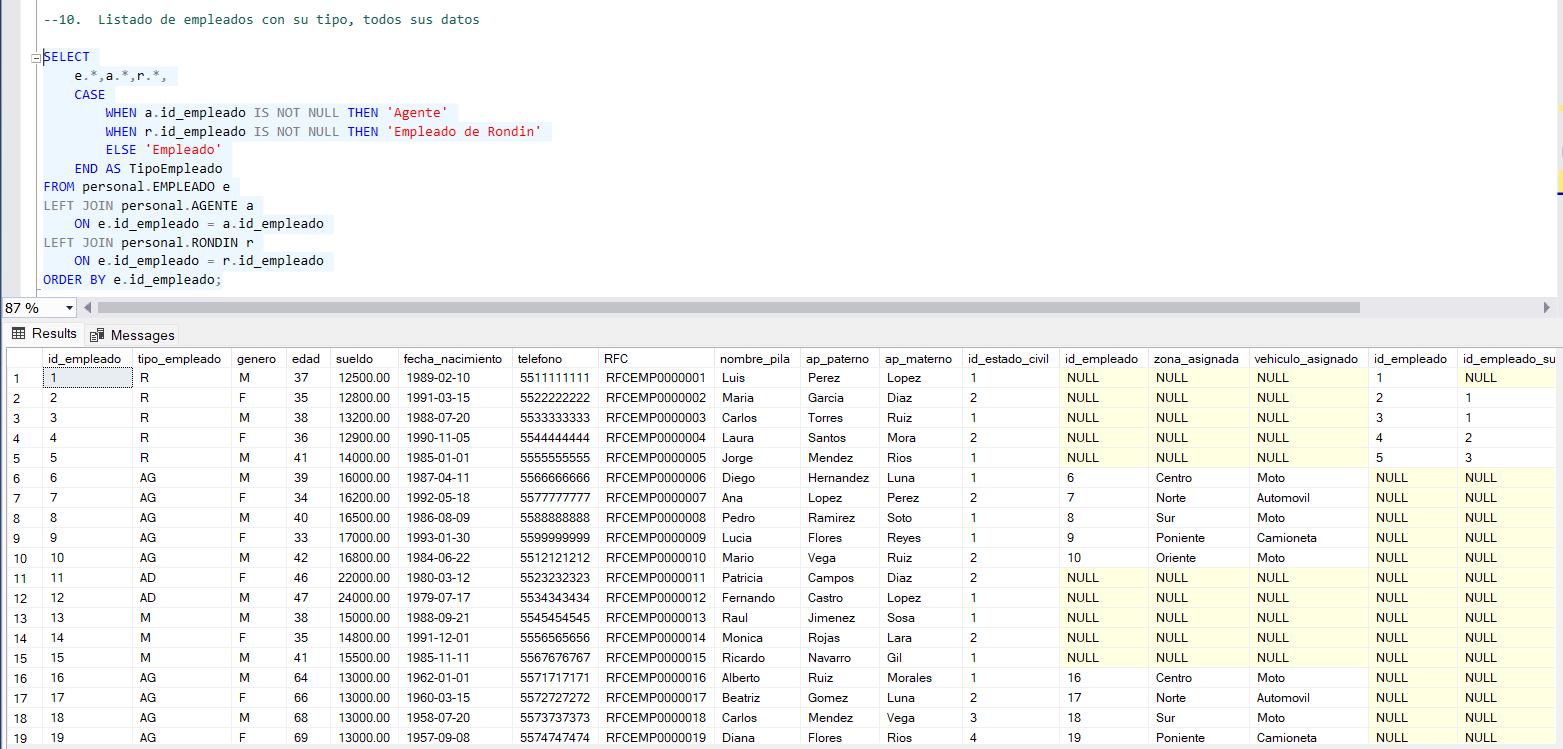
\includegraphics[width=0.85\textwidth]{figures/fig-013.png}
	\caption{Listado completo de empleados}
	\label{fig:est_10}
\end{figure}

\subsection{Estadística 11. Informe de recorridos}

Esta consulta genera un informe detallado de los viajes realizados por los usuarios, incluyendo estaciones de origen y destino, duración del recorrido y costo generado, en un periodo y/o estación determinada.

\begin{figure}[H]
	\centering
	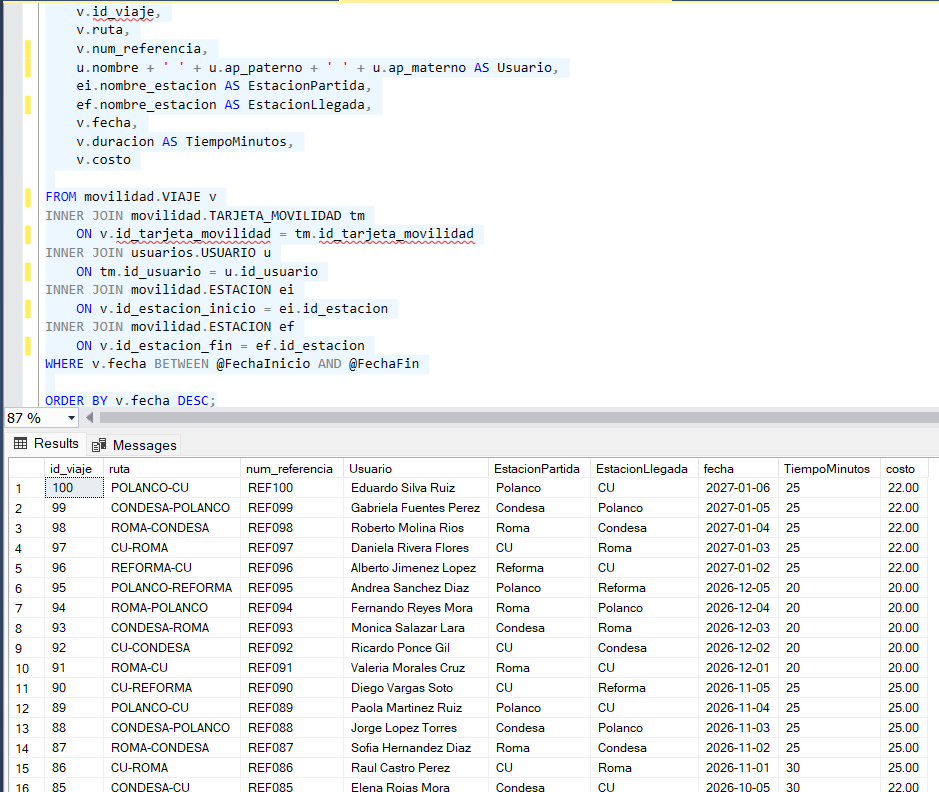
\includegraphics[width=0.85\textwidth]{figures/fig-014.png}
	\caption{Informe de recorridos}
	\label{fig:est_11}
\end{figure}

\subsection{Estadística 12. Recorridos por temporada}

Esta consulta permite conocer la cantidad de recorridos realizados durante cada temporada o época del año, identificando los periodos de mayor actividad ordenados de mayor a menor.

\begin{figure}[H]
	\centering
	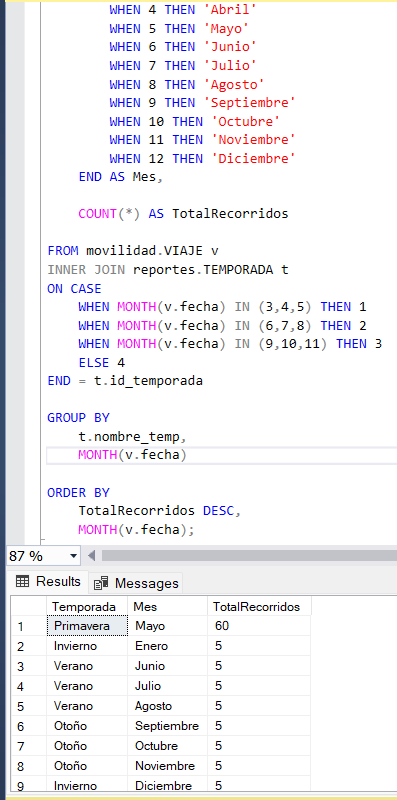
\includegraphics[width=0.85\textwidth]{figures/fig-015.png}
	\caption{Recorridos por temporada}
	\label{fig:est_12}
\end{figure}

\subsection{Estadística 13. Accidentes atendidos por agente}

Esta consulta muestra los datos personales de cada agente y el historial de accidentes que ha atendido, incluyendo fecha, lugar y tipo de incidente.

\begin{figure}[H]
	\centering
	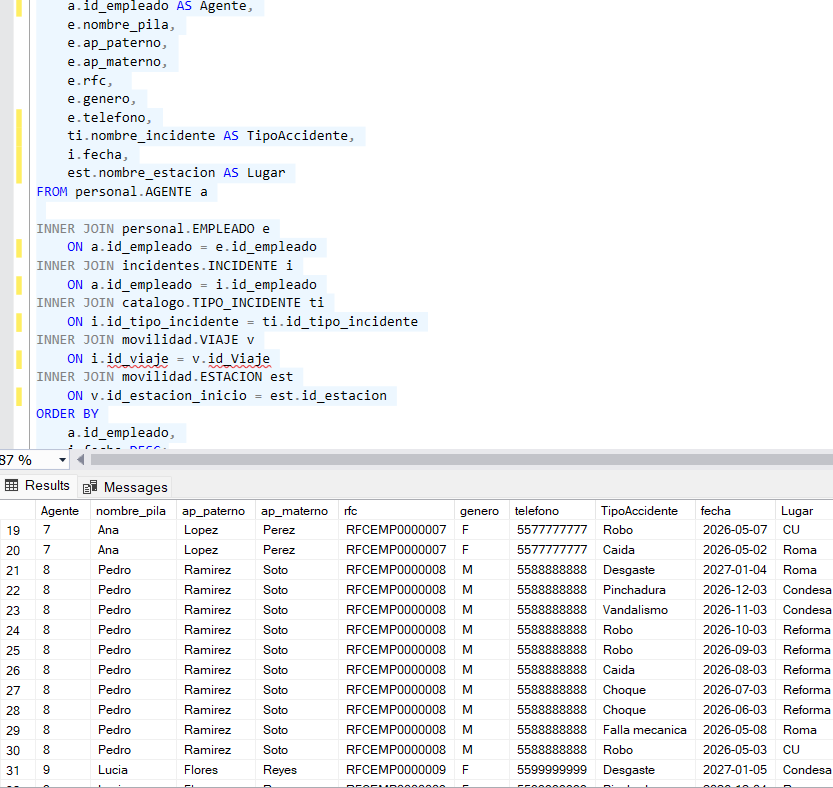
\includegraphics[width=0.85\textwidth]{figures/fig-016.png}
	\caption{Accidentes atendidos por agente}
	\label{fig:est_13}
\end{figure}

\subsection{Estadística 14. Informe de Recursos Humanos}

Esta consulta identifica empleados del área de administración que son de la tercera edad y que perciben un sueldo mensual de \$13,000, apoyando los procesos de análisis y gestión de recursos humanos.

\begin{figure}[H]
	\centering
	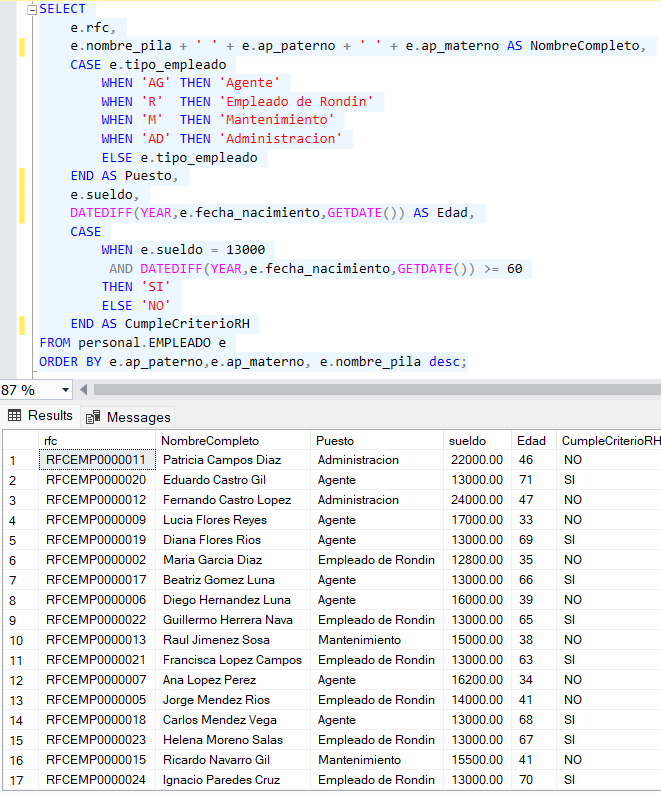
\includegraphics[width=0.85\textwidth]{figures/fig-017.png}
	\caption{Informe de Recursos Humanos}
	\label{fig:est_14}
\end{figure}

\subsection{Estadística 15. Faltas de empleados}

Esta consulta presenta estadísticas de faltas de empleados por periodo, clasificadas según el motivo registrado. La información permite analizar patrones de ausentismo dentro de la organización.

\begin{figure}[H]
	\centering
	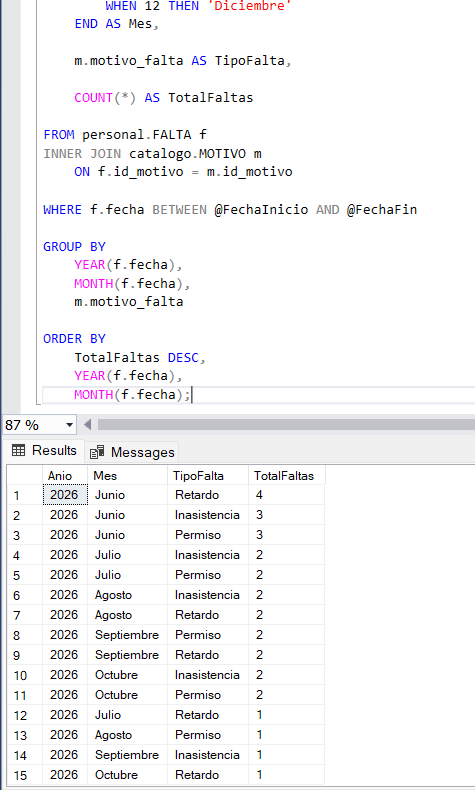
\includegraphics[width=0.85\textwidth]{figures/fig-018.png}
	\caption{Faltas de empleados}
	\label{fig:est_15}
\end{figure}
